\documentclass[12pt]{report}

\usepackage[english]{babel}
\usepackage[utf8x]{inputenc}
\usepackage{amsmath}
\usepackage{graphicx}
\usepackage{multirow}
\usepackage[hypcap]{caption}
\usepackage{setspace} 
\usepackage{float}

\title{Lab 8: Polymers}
\author{Zachary Tschirhart \\
	\small \\
        \small EID: zst75 \\
	\small Department of Aerospace Engineering and Engineering Mechanics \\
	\small \textbf{ASE 324L (Mon 2:00-5:00)} \\
	\small Unique: 13740}
\date{April 1, 2014}


\begin{document}
\maketitle

\setcounter{secnumdepth}{0}

\section{Results and Discussion}
\doublespacing

\subsection{Question 1}

The necking between the two materials is different, in strength and the area that it occurs. When the polymers begin to neck, they form stable necks. This is because the polymer chains are stretched and are aligned. The necks produced by steel and aluminum alloy do not align the carbon chains. Another difference is the strength during necking, polymers increase there strength almost exponentially at the end of their necking region. Steel and aluminum usually decrease strength toward the end of their necking region. Lastly, when the polymer specimen is unloaded, the stress-strain curve does not follow a linear back down to zero stress. The steel and aluminum specimen do follow a linear curve back to zero stress when unloaded.

\subsection{Question 2}
\begin{figure}[H]
	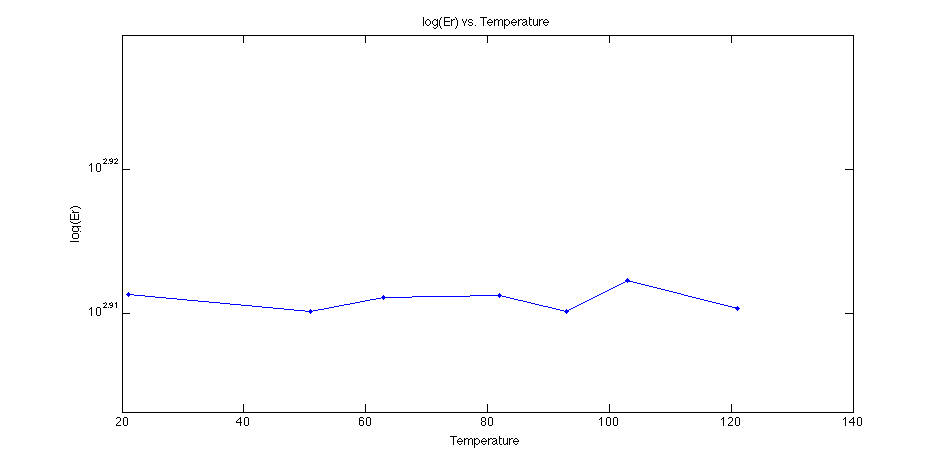
\includegraphics[width=1\textwidth]{problem2.png}
	\caption{Semilog scale of temperature versus relaxation modulus.}
	\label{fig:Figure1}
\end{figure}

\subsection{Question 3}
\begin{figure}[H]
	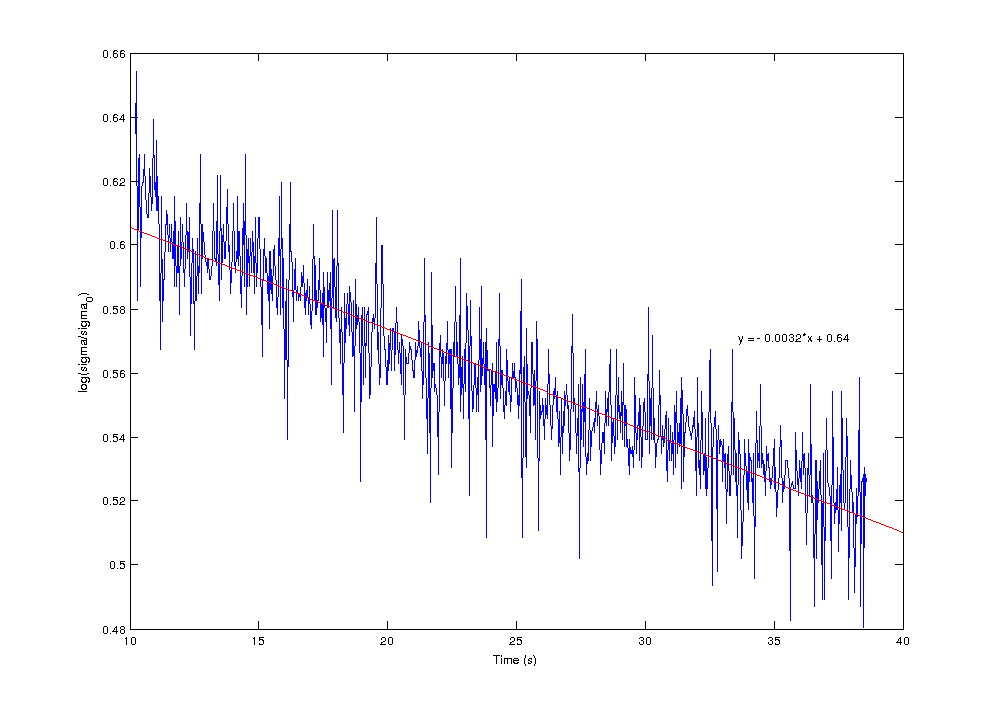
\includegraphics[width=1\textwidth]{problem3.png}
	\caption{stress relaxation data used to construct a Maxwell model.}
	\label{fig:Figure2}
\end{figure}

The viscosity was determined by taking the negative inverse of the slope, and multiplying by the E0. This came out to be 2.19345E6 psi-s. The spring constant based on the stress relaxation curve was 5.70626E4 psi.

\subsection{Question 4}
Derivation attached

\subsection{Question 5}
Derivation attached

\subsection{Question 6}
Polymers exhibit crystallinity after cooling down after melting or stretching of the polymer. To distinguish between crystalline and amorphous polymers using volume change measurements, a criteria is needed to establish a difference. The difference between the two polymer types is density, crystalline areas are generally more densely packed than amorphous areas. Since density is a function of volume and mass, and mass is not changing, then volume changes can determine density changes. This can be used to determine the difference between the two.
\end{document}
